% Created: Enze Chen, June 2017
% Last edited: Enze Chen, December 2017
%
% Chapter 3 of the MSE 142 coursereader. This chapter discusses the particle in a box model as a concrete application of the time-independent Schrodinger equation. Quantization, normalization, and the uncertainty principle are discussed. This model is a good approximation for quantum dots, our first physical example of a quantum mechanical system.

% Uncomment the following three lines and last line to individually compile this chapter
%\documentclass[12pt, english]{book}
%\usepackage{142crstyle}
%\begin{document}

\chapter{Particle In A Box} \label{ch:box}
%{ \doublespacing 
In the previous chapter, we derived the \Sch\ equation, which provides the theoretical underpinning for all quantum mechanical calculations. Now we will apply the \Sch\ equation to a simple example and solve for the wave function $\Psi$. This will give us a better understanding of the mathematical constructs we saw previously and how they can be applied to a physical system like quantum dots.

\section{Formulation}
As its name would imply, the \textbf{particle in a box} model is just that: we have a small particle (e.g. an electron) that is free to move in one dimension in a small space confined between $x=0$ and $x=L$ (Figure~\ref{fig:box}). In order to keep the particle confined, we imagine the potential $V$ to be $\infty$ outside of the walls and 0 on the inside. For this reason, this model is also known as the \textbf{infinite potential well}. Physically, you can think of this as a guitar string of length $L$ with the two ends fixed in place so that it cannot vibrate at the ends.

\begin{figure}[!h]
	\centering
	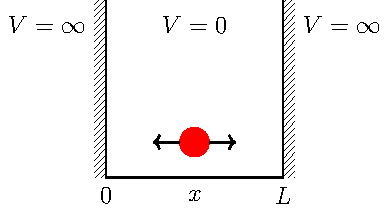
\includegraphics[width=0.45\linewidth]{particle-in-a-box}
	\caption{Particle in a box model. The potential $V(x)$ is zero for $x\in[0,L]$ and infinite everywhere else, which confines the movement of the particle to be inside the walls at all times.}
	\label{fig:box}
\end{figure}

The particle in a box model is a great starting point for us because it is simple enough to be solved analytically to illustrate all sorts of amazing quantum behavior. We first enforce the condition that the wave function $\Psi(x,t)$ must be zero at $x=0$ and $x=L$ for all time $t$. This means the probability of finding the particle there is zero, which makes sense given the infinite potential barriers. \par 

Inside the box, where $V(x) = 0$, the time-independent \Sch\ equation (Equation~\ref{eq:tise}) now adopts the simplified form
\begin{tcolorbox}[title=\Sch\ equation for particle in a box] \vspace{-2ex}
	\begin{equation}
		-\frac{\hbar^2}{2m} \dv[2]{\psi_n}{x} = E_n\psi_n  \label{eq:box-se}
	\end{equation}
\end{tcolorbox}
where we have again explicitly put the index $n$ to label different solutions for different quantum states. Now we are looking for a function with which two derivatives will give us back the original function times a negative constant. Equation~\ref{eq:box-se} is actually the equation for a simple harmonic oscillator from classical mechanics, which you might recall has sines and cosines as solutions.\footnote{Alternatively, employ the method of educated guessing as we showed in class to arrive at this result.} In fact, the general solution is given by 
\begin{tcolorbox}[title=General solution to particle in a box] \vspace{-2ex}
	\begin{equation}
		\psi_n(x) = A\sin(k_nx) + B\cos(k_nx) \label{box-gensol}
	\end{equation}
\end{tcolorbox}
where $k_n = \sqrt{2mE_n/\hbar^2}$ and $A$ and $B$ are arbitrary constants. We definitely took a big jump going directly from Equation~\ref{eq:box-se} to~\ref{box-gensol}, so if you're not quite convinced, I recommend plugging the latter equation into the former to make sure that it is indeed a valid solution.

%%%%%%%%%%%%%%%%%%%%%%%%%%%%%%%%%%%%%%%%%%%%%%%%%%%%%%%%%%%%%%%%%%%%%%%%%%%%%%%%

\section{Quantization}
With the general solution on hand, we now look to see if the constraints in the problem can help us simplify some of the constants. Typically, the constants that appear in solutions to differential equations are fixed by the \textbf{boundary conditions} of the problem. We already noted earlier that
\begin{align}
	\psi(0) &= 0 \\
	\psi(L) &= 0
\end{align}
which seem appropriate for this model. From the first boundary condition, we have
\begin{equation*}
	\psi(0) = A\sin(k_n \cdot 0) + B\cos(k_n \cdot 0) = B = 0
\end{equation*}
which means the cosine term is eliminated! From the second boundary condition, we have
\begin{equation*}
	\psi(L) = A\sin(k_nL) = 0
\end{equation*}

This scenario is slightly trickier, but realize that we cannot have $A=0$ and still have a physically meaningful solution, so we must have $\sin(k_nL) = 0$. Since the sine function has roots at integer multiples of $\pi$, this means that
\begin{equation}
	k_nL = 0,\ \pm\pi,\ \pm2\pi,\ \pm3\pi,\ \dots \label{eq:k-pi-box}
\end{equation}

Analyzing Equation~\ref{eq:k-pi-box} closely, we can argue that $k=0$ would also lead to a trivial solution and we can eliminate the negative solutions due to symmetry, given that $\sin(-k_nL) = -\sin(k_nL)$ would give us the same wave function up to a sign. Therefore, it must be the case that 
\begin{tcolorbox}[title=Allowed values of $k$] \vspace{-2ex}
	\begin{equation}
		k_n = \frac{n\pi}{L}, \quad n = 1, 2, 3, \dots   \label{eq:k-box}
	\end{equation}
\end{tcolorbox}

Now you see why we chose to index the solutions with the subscript $n$ all along. Furthermore, because $k_n = \sqrt{2mE_n/\hbar^2}$, we can use some algebra and find that 
\begin{tcolorbox}[title = Allowed energies] \vspace{-2ex}
	\begin{equation}
		E_n = \frac{\hbar^2n^2\pi^2}{2mL^2} \label{eq:E-box}
	\end{equation}
\end{tcolorbox}

The results from these two expressions show that the energy states of a particle in an infinite potential well are not a continuum of values but rather a set of discrete energy levels. Thus we say that the energies for a particle in a box are \textbf{quantized}, where each state is indexed by the \textbf{quantum number} $n$. We see then that $n=1$ corresponds to the lowest energy state, called the \textbf{ground state} of the system, and higher energy states are called \textbf{excited states} (analogous to harmonics in music). Note how strange this is: Whereas classically, a particle can have zero total energy, here we are saying that is not the case, even for the ground state!\footnote{We will elaborate on this further in Chapter~\ref{ch:qho} when we discuss the zero-point energy of the quantum harmonic oscillator.} 

%%%%%%%%%%%%%%%%%%%%%%%%%%%%%%%%%%%%%%%%%%%%%%%%%%%%%%%%%%%%%%%%%%%%%%%%%%%%%%%%

\section{Normalization}
Now that we have an expression for $k_n$ and cleverly eliminated $B$, all that's left is to find the leading coefficient $A$. Recall how in Section~\ref{sec:normse} we used the normalization condition to help us with this task, so let's apply that again here. Specifically, we have
\begin{align*}
	\int_0^L \abs{A}^2 \sin^2(k_nx)\dd{x} &= 1 \\
	\abs{A}^2 \int_0^L \sin^2\left(\frac{n\pi x}{L}\right)\dd{x} &= 1 \\ 
	\abs{A}^2 \int_0^L \frac{1}{2} - \frac{1}{2}\cos\left(\frac{2n\pi x}{L}\right)\dd{x} &= 1 \\
%	\abs{A}^2 \left( \frac{L}{2} - \frac{L}{4n\pi}(\sin(2n\pi) - \sin(0)) \right) &= 1 \\
	\abs{A}^2 \left(\frac{L}{2}\right) &= 1 \\
	\abs{A}^2 &= \frac{2}{L}
\end{align*}
where we have used the trigonometric identity $\sin^2(x) = \frac{1}{2}\left(1 - \cos(2x)\right)$ going from the second line to the third line. We take the positive real root to get $A = \sqrt{2/L}$. Inside the confines of the box, we have the stationary state solutions given by 
\begin{tcolorbox}[title=Stationary state solutions] \vspace{-2ex}
	\begin{equation}
		\psi_n(x) = \sqrt{\frac{2}{L}} \sin \left(\frac{n\pi x}{L}\right) \label{eq:box-ss}
	\end{equation}
\end{tcolorbox}

The first three stationary states are plotted in Figure~\ref{fig:ss-box}, and they look similar to the standing waves we observe when we pluck a guitar string.\footnote{In fact, the superposition of the various harmonics in musical instruments is what gives each instrument its unique timbre, or tone quality.} We will call zero-crossings on the wave function \textbf{nodes}, which means the $n$th quantum state has $n-1$ nodes (alternatively, the $n$th \emph{excited} state has $n$ nodes). These nodes restrict the location where the particle may be found and contribute to the symmetry of the wave functions.

\begin{figure}[!h]
	\centering
	\subfloat[]{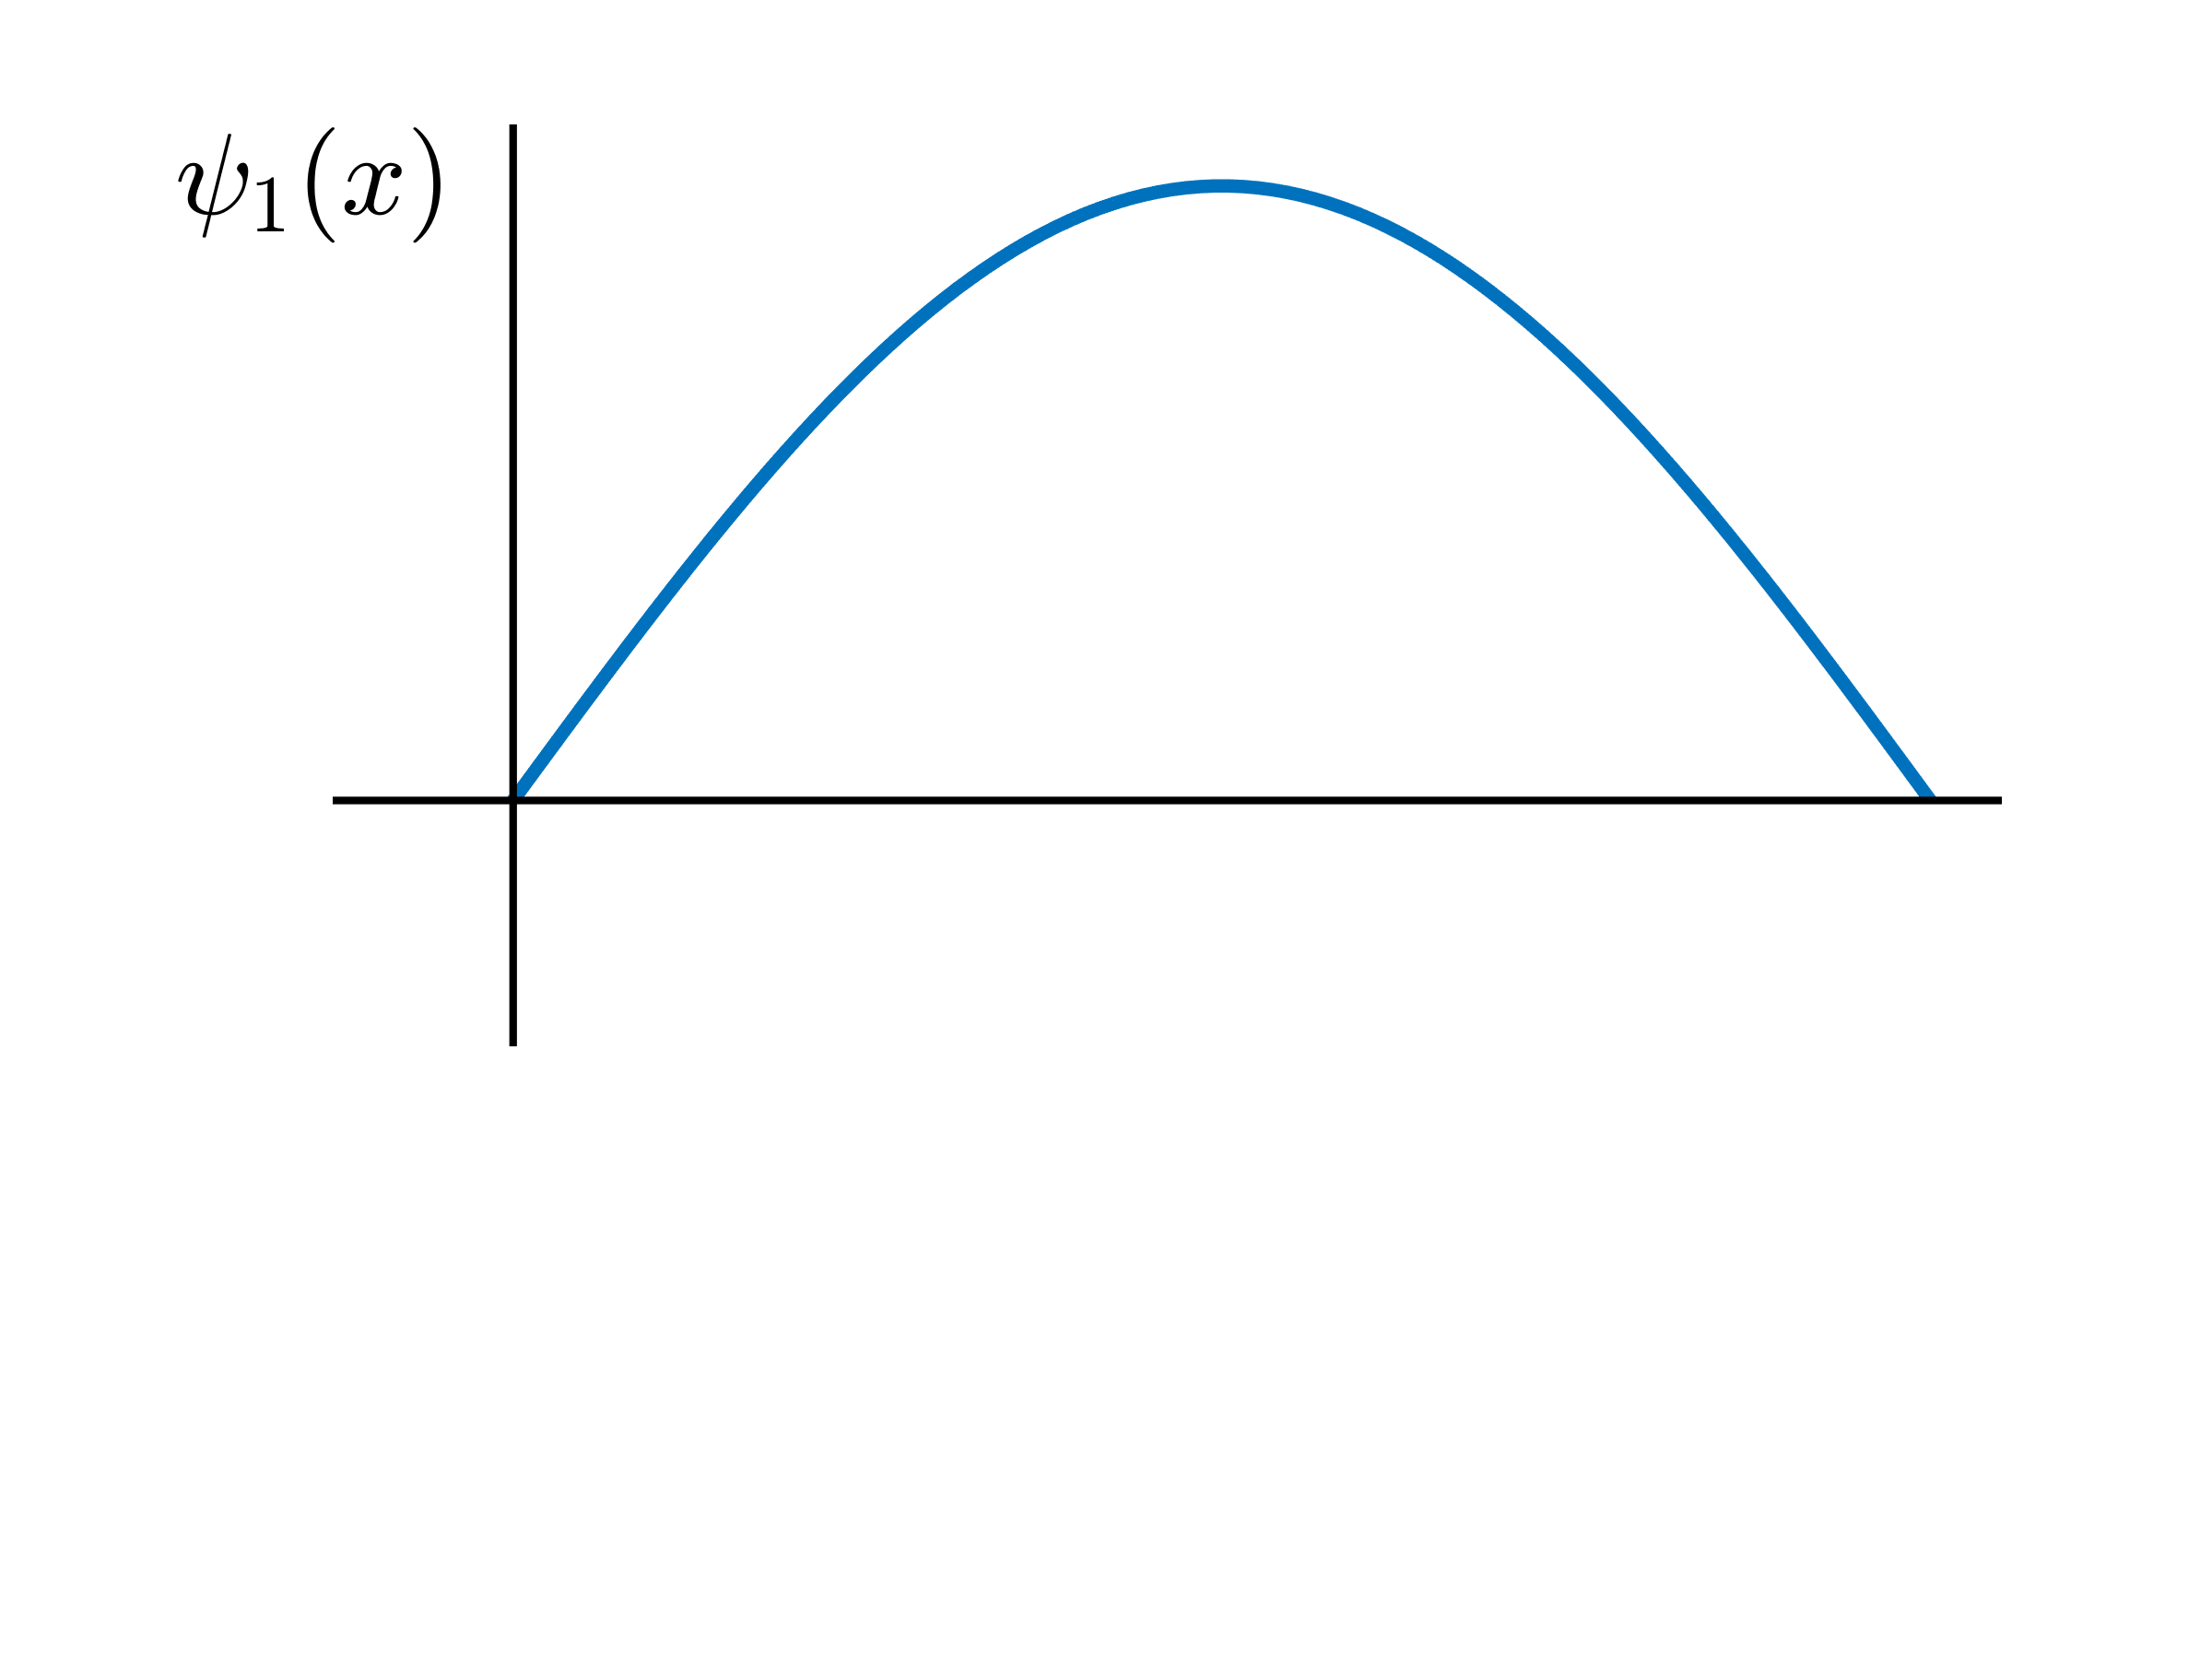
\includegraphics[width=0.33\linewidth]{ss-1}}
	\subfloat[]{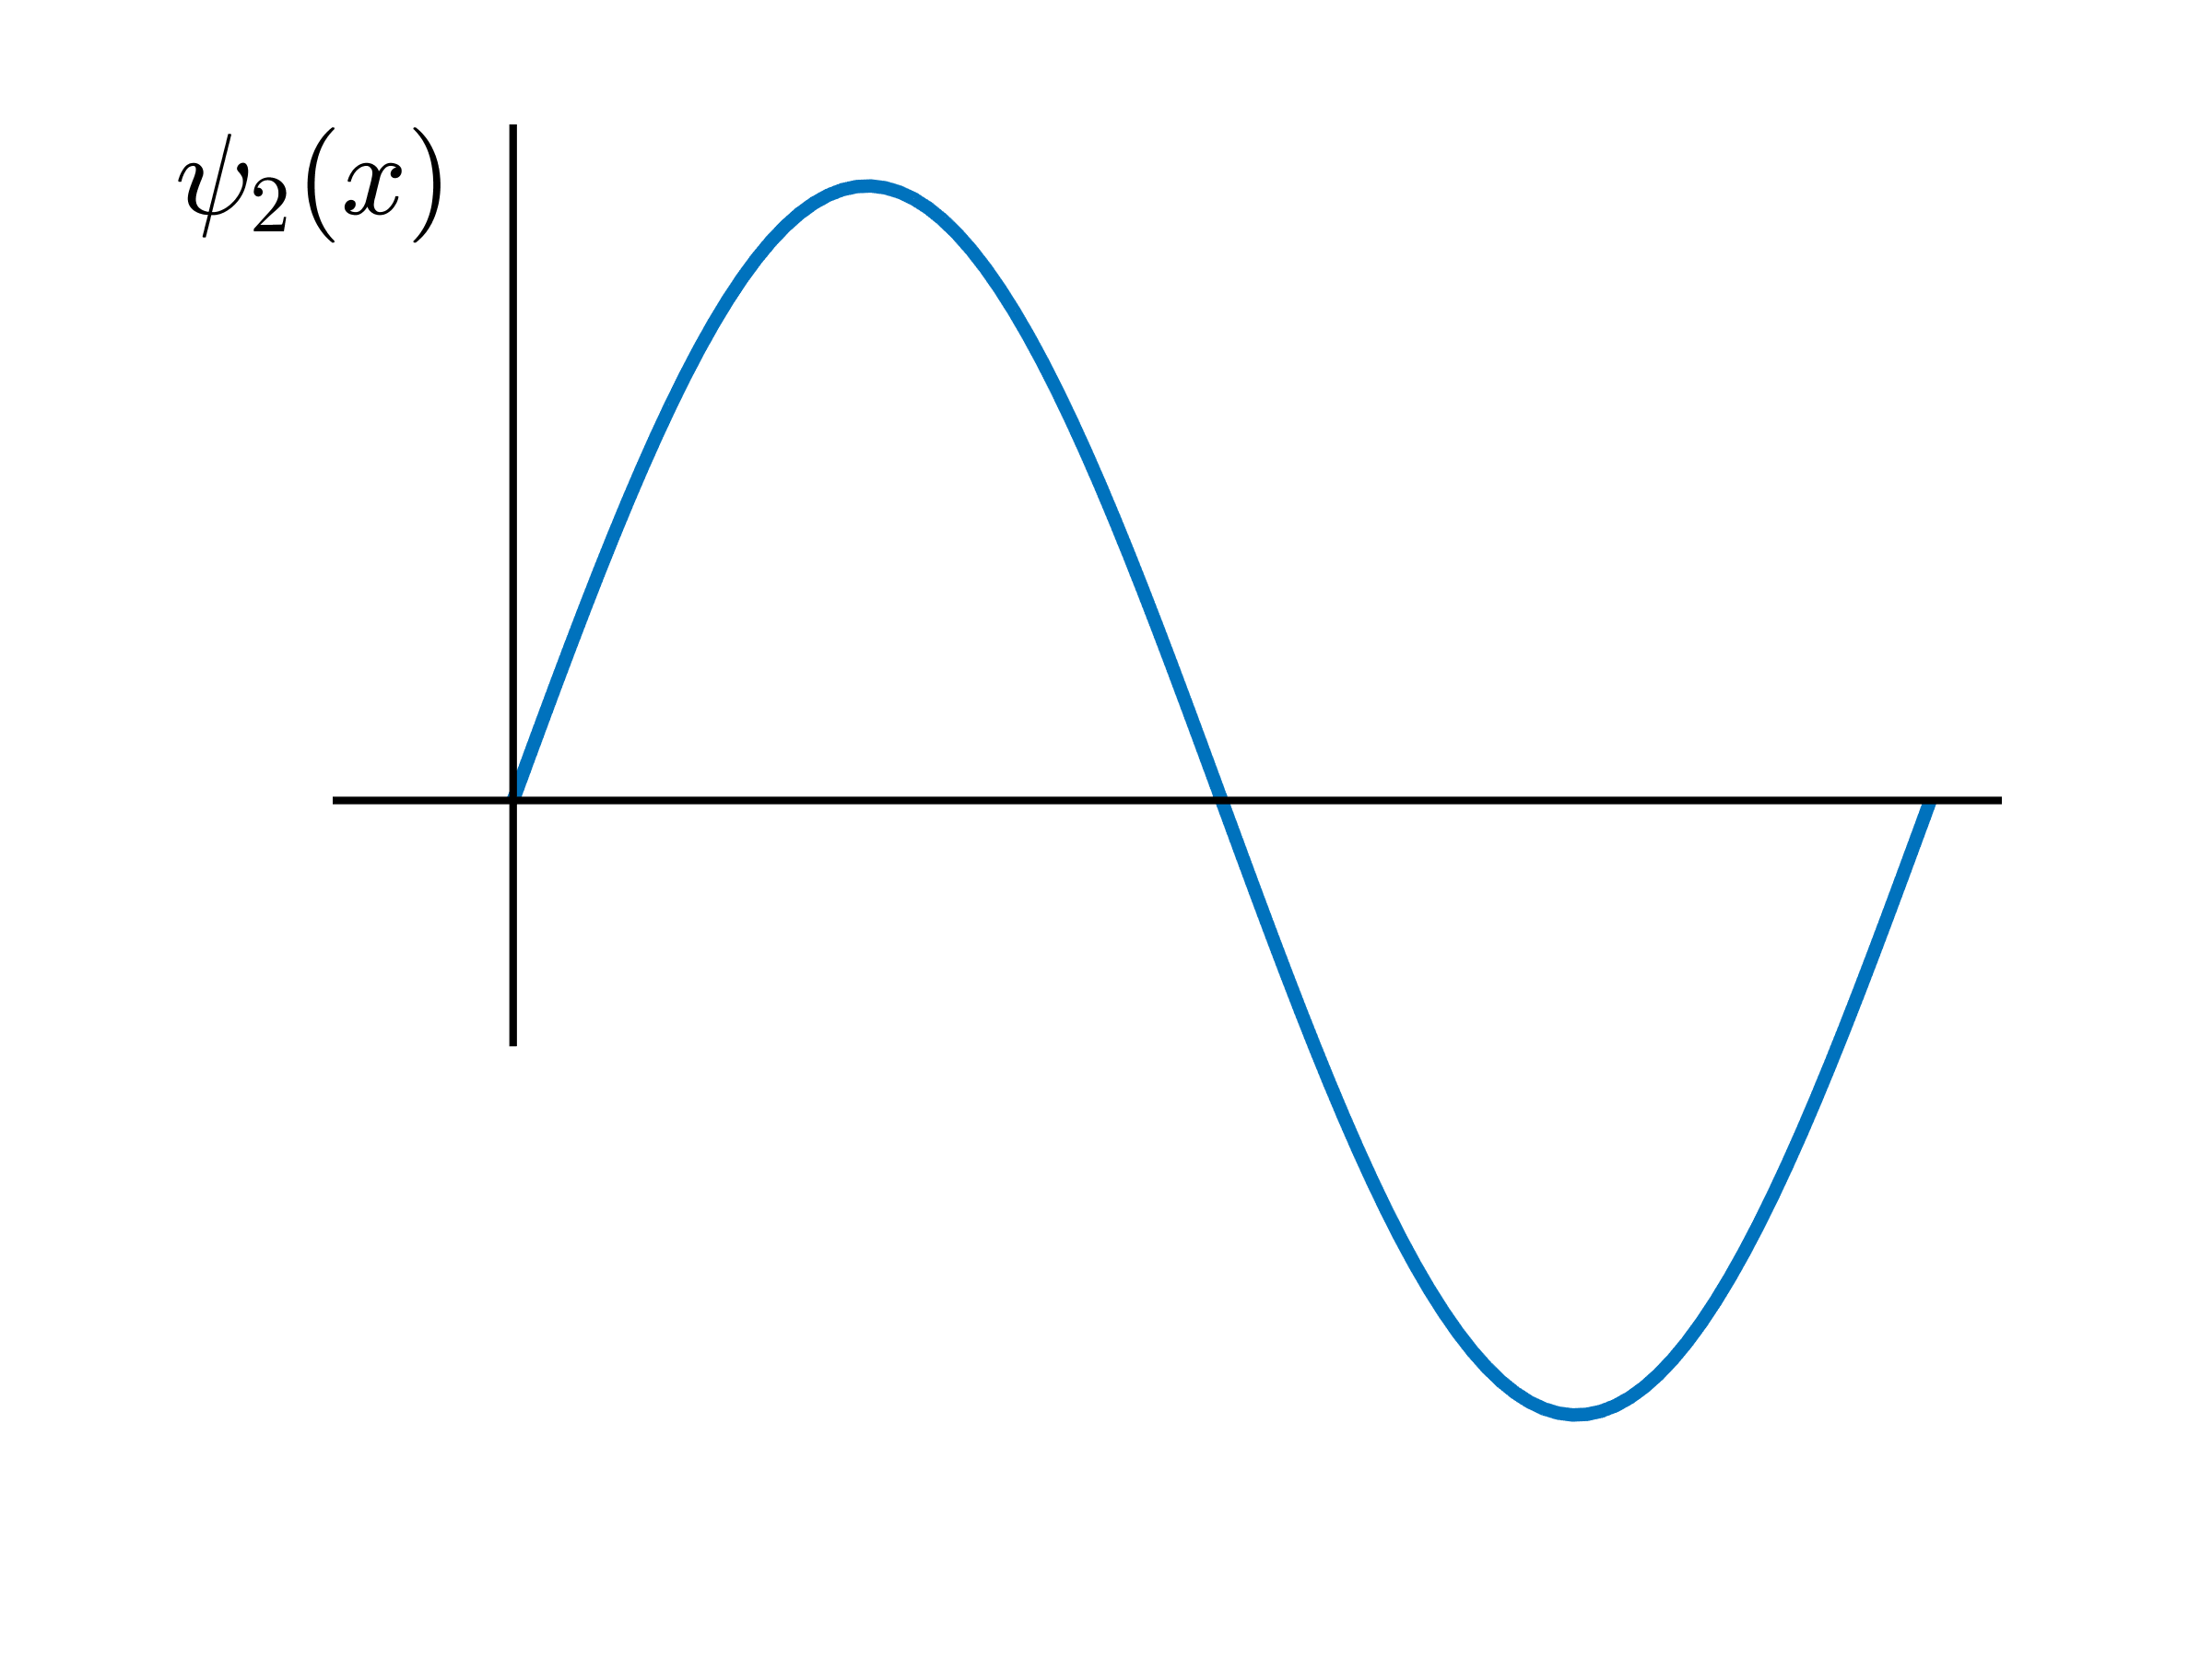
\includegraphics[width=0.33\linewidth]{ss-2}}
	\subfloat[]{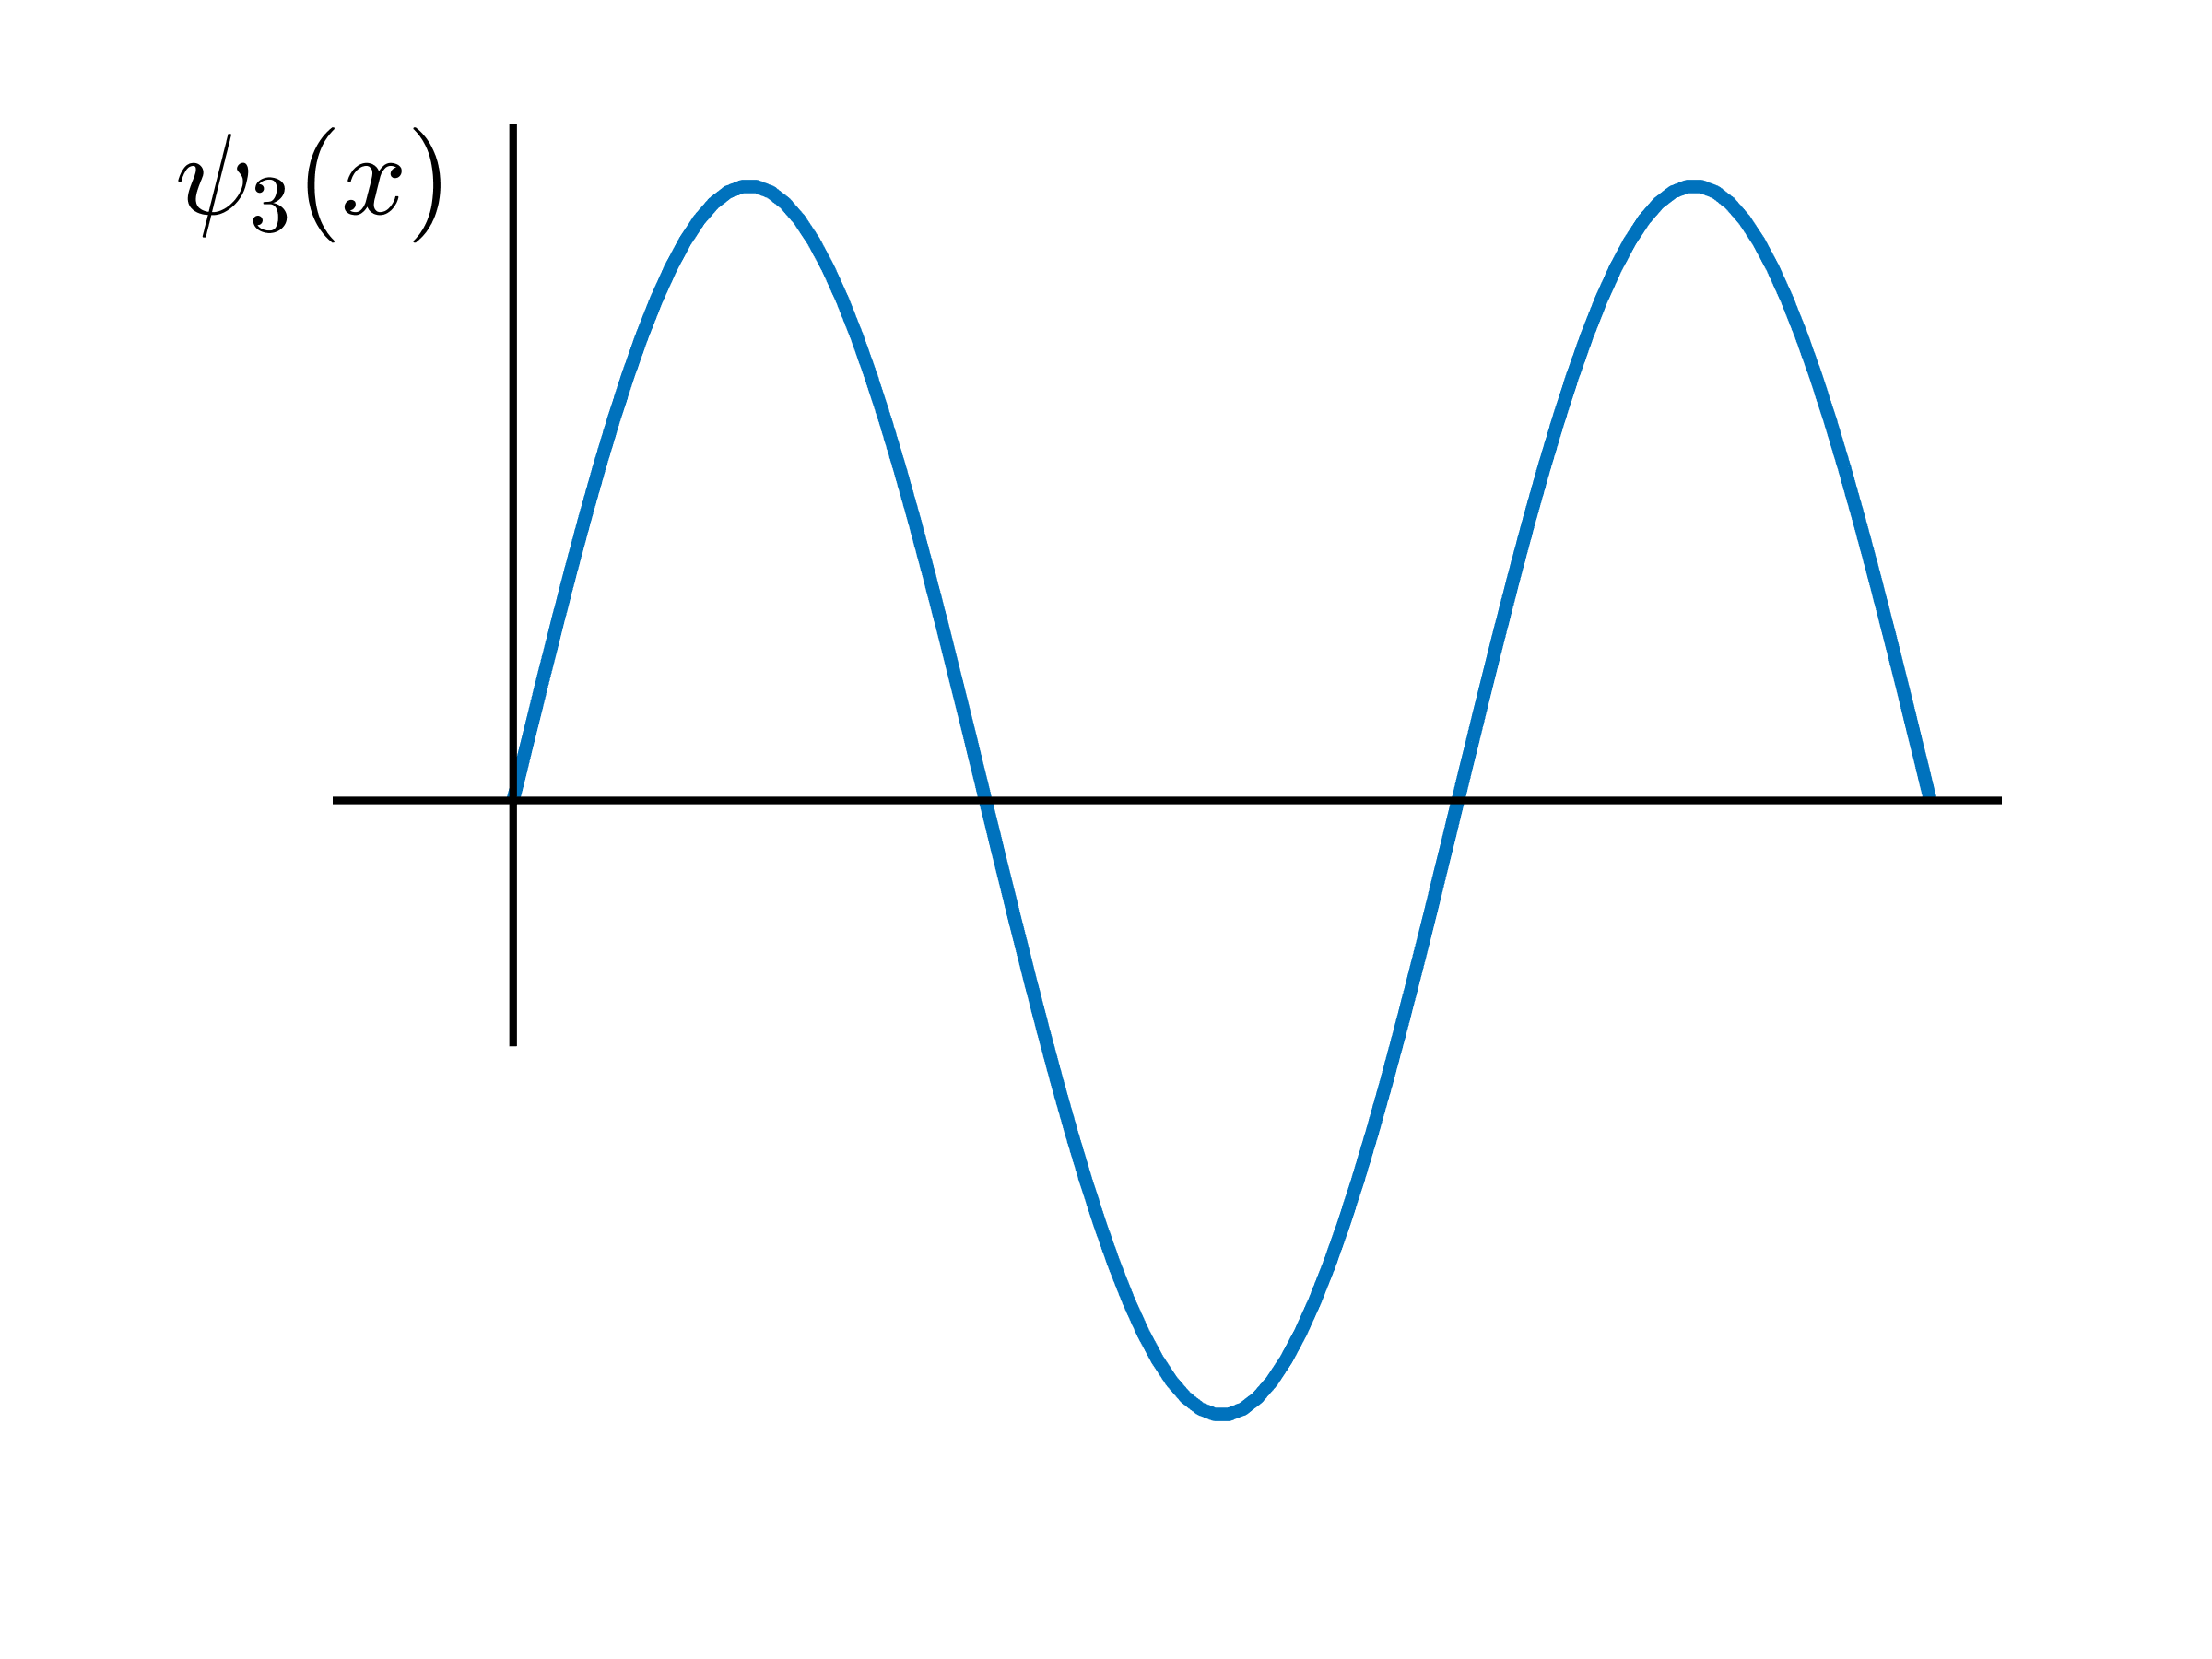
\includegraphics[width=0.33\linewidth]{ss-3}}
	\caption{The first three stationary states of the particle in a box model.}
	\label{fig:ss-box}
\end{figure}

%%%%%%%%%%%%%%%%%%%%%%%%%%%%%%%%%%%%%%%%%%%%%%%%%%%%%%%%%%%%%%%%%%%%%%%%%%%%%%%%

\section{Orthogonality}
Another interesting property of the wave functions given by Equation~\ref{eq:box-ss} is that they are all mutually orthogonal. This means 
\begin{equation*}
	\int \psi_m^*(x) \psi_n(x) \dd{x} = 0, \quad \forall m \neq n
\end{equation*}
where $\psi^*$ again denotes the complex conjugate. We will show this as follows:
\begin{align*}
	\int \psi_m^*(x) \psi_n(x) \dd{x} &= \frac{2}{L} \int_0^L \sin\left(\frac{m\pi x}{L}\right) \sin\left(\frac{n\pi x}{L} \right) \dd{x} \\
	&= \frac{1}{L} \int_{0}^{L} \left[ \cos\left(\frac{(m-n)\pi x}{L}\right) - \cos\left(\frac{(m+n)\pi x}{L}\right) \right] \dd{x} \\
	&= \left[ \frac{1}{(m-n)\pi} \sin \left(\frac{(m-n)\pi x}{L}\right) - \frac{1}{(m+n)\pi} \sin\left( \frac{(m+n)\pi x}{L} \right)\right] \bigg|_0^L \\
	&= \frac{1}{\pi} \left( \frac{\sin((m-n)\pi)}{m-n} - \frac{\sin((m+n)\pi)}{m+n}\right) \\
	&= 0 \tag{when $m\neq n$, $\{m,n\} \in \mathbb{Z}$}
\end{align*}
where we used the identity $\sin(m)\sin(n) = \frac{1}{2}(\cos(m-n) - \cos(m+n))$ in the second line. That's pretty neat! We do note, however, the special case when $m=n$. In that case, by the normalization condition, the integrand is equivalent to the probability density function, which we know equals 1 when integrated over the range of $x$. This fact allows us to combine orthogonality and normalization into a single expression.
\begin{tcolorbox}[title = Orthonormal stationary states] \vspace{-2ex}
	\begin{equation}
		\int \psi_m^*(x) \psi_n(x) \dd{x} = \delta_{mn}\ \begin{cases}
		1 & \text{if}\ m=n \\
		0 & \text{if}\ m\neq n
		\end{cases} \label{eq:orthonorm}
	\end{equation}
\end{tcolorbox}
where $\delta_{mn}$ is known as the \textbf{Kronecker delta} function. Now we have confirmed that the $\psi$'s form an \textbf{orthonormal basis}, which allows us to express \emph{any} function as a linear combination of them.\footnote{I wanted correctness here, but this is excessive linear algebra jargon. A simple example of an orthonormal basis is the set of unit vectors $\mathbf{i}$, $\mathbf{j}$, $\mathbf{k}$ in $(x,y,z)$ coordinates. Every point in 3D space is some linear combination of the three unit vectors and each unit vector is orthogonal to the others.} Thus, we can write down the full, time-dependent solution for the particle in a box as:
\begin{equation}
	\Psi(x,t) = \sum_{n=1}^{\infty} A_n \sin \left(\frac{n\pi x}{L}\right) e^{-iE_nt/\hbar} \label{eq:tdwf-box}
\end{equation}

This equation gets us very close to the general solution, but we still have $A_n$ to solve for---and that's where the following ``mathematical trick'' comes in. We noted in Section~\ref{sec:normse} how $A_n$ is time-invariant, so let's look at our wave function at time $t=0$. From Equation~\ref{eq:tdwf-box}, we obtain
\begin{equation*}
	\Psi(x,0) = \sum_{n=1}^{\infty} A_n \sin \left(\frac{n\pi x}{L} \right)
\end{equation*}
where the exponential term has dropped out. Now for the ``trick'': It would appear that this is still an infinite sum of sine terms, but we can make use of Equation~\ref{eq:orthonorm} by multiplying both sides by an arbitrary function $\sin \left(\frac{j\pi x}{L}\right)$ and then integrating the result.\footnote{This is definitely \emph{not} obvious, and is a technique borrowed directly from Fourier Series (see \href{http://tutorial.math.lamar.edu/Classes/DE/FourierSeries.aspx}{Paul Dawkins'} page if you're curious). You don't need to know this trick per se, but do understand why it works (aka, Equation~\ref{eq:orthonorm}).} This gives us
\begin{align*}
	\Psi(x,0) &= \sum_{n=1}^{\infty} A_n \sin \left(\frac{n\pi x}{L} \right) \\
	\int_0^L \Psi(x,0) \sin \left(\frac{j \pi x}{L}\right) \dd{x} &= \int_0^L \sum_{n=1}^{\infty} A_n \sin \left(\frac{n\pi x}{L} \right) \sin \left( \frac{j \pi x}{L}\right) \dd{x} \\
	\int_0^L \Psi(x,0) \sin \left(\frac{j \pi x}{L}\right) \dd{x} &= \sum_{n=1}^{\infty} A_n \int_0^L \sin \left(\frac{n\pi x}{L} \right) \sin \left( \frac{j \pi x}{L}\right) \dd{x} \\
	\int_0^L \Psi(x,0) \sin \left(\frac{j \pi x}{L}\right) \dd{x} &= \sum_{n=1}^{\infty} A_n \delta_{nj} \frac{L}{2}
\end{align*}

The right hand side is 0 for all values of $n$ except when $n=j$. Thus the summation is eliminated and we can move $\frac{L}{2}$ to the other side (and change $j$ to $n$) to obtain
\begin{tcolorbox}[title = Wave function expansion coefficients] \vspace{-2ex}
	\begin{equation}
		A_n = \frac{2}{L} \int_0^L \Psi(x,0) \sin \left(\frac{n\pi x}{L}\right) \dd{x} \label{eq:wf-coeff}
	\end{equation}
\end{tcolorbox}

Whew! After some nifty math, we were finally able to derive a general solution to the \Sch\ equation given the stationary state solutions from our particle in a box model. The general solution is given by Equation~\ref{eq:tdwf-box} and those coefficients $A_n$ are described by Equation~\ref{eq:wf-coeff} provided we are given some initial condition $\Psi(x,0)$.

%%%%%%%%%%%%%%%%%%%%%%%%%%%%%%%%%%%%%%%%%%%%%%%%%%%%%%%%%%%%%%%%%%%%%%%%%%%%%%%%

\section{Uncertainty principle}
Let's try to calculate the amplitude coefficients using Equation~\ref{eq:wf-coeff} for a simple case and arrive at another fundamental principle in quantum mechanics. First, we assume that our wave function has the initial profile shown in Figure~\ref{fig:square-box}. That is, it is a square wave of height $A$ and width $b$ centered in the middle of the infinite potential well.

\begin{figure}[!h]
	\centering
	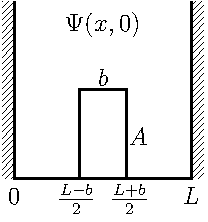
\includegraphics[width=0.26\linewidth]{square-box}
	\caption{Initial wave function profile of height $A$ and width $b$ centered in the middle of the well.}
	\label{fig:square-box}
\end{figure}

We directly crank through the calculations in Equation~\ref{eq:wf-coeff} to obtain:
\begin{align*}
	A_n &= \frac{2}{L} \int_0^L \Psi(x,0) \sin \left(\frac{n\pi x}{L}\right) \dd{x} \\
	&= \frac{2A}{L} \int_{(L-b)/2}^{(L+b)/2} \sin \left(\frac{n\pi x}{L}\right) \dd{x} \\
	&= -\frac{L}{n\pi}\frac{2A}{L} \cos\left(\frac{n \pi x}{L}\right)\bigg|_{(L-b)/2}^{(L+b)/2} \\
	&= \frac{2A}{n\pi} \left[ \cos \left(\frac{L-b}{2}\frac{n\pi}{L}\right) - \cos \left(\frac{L+b}{2}\frac{n\pi}{L}\right) \right] \\
	&= \frac{4A}{n\pi} \sin \left(\frac{n\pi}{2}\right) \sin \left(\frac{n\pi b}{2L}\right) \\
	&= \frac{4A}{n\pi} (-1)^{\frac{n-1}{2}} \sin \left(\frac{n\pi b}{2L}\right) \tag{for odd $n$} \\
	&= \frac{4A(b/2L)}{n\pi(b/2L)} (-1)^{\frac{n-1}{2}} \sin \left(\frac{n\pi b}{2L}\right) \\
	\Aboxed{A_n &= \frac{2Ab}{L} (-1)^{\frac{n-1}{2}} \frac{\sin \left(k_nb/2\right)}{k_nb/2}} \numberthis \label{eq:A-example}
\end{align*}


Notice how we used the same trigonometric identity as before, $\sin(m)\sin(n) = \frac{1}{2}(\cos(m-n) - \cos(m+n))$, except backwards, when we went from the fourth line to the fifth line. The second to last line involves multiplying by ``1'' so that we can get the final answer in the form of $\frac{\sin(x)}{x}$. This allows us to analyze Equation~\ref{eq:A-example} in the form of a plot, which is shown in Figure~\ref{fig:sinx/x}.

\begin{figure}[!h]
	\centering
	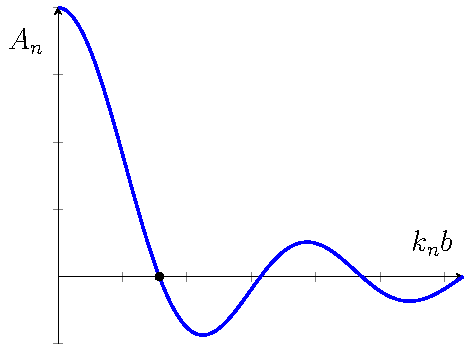
\includegraphics[width=0.35\linewidth]{sinx-x}
	\caption{A basic sketch of Equation~\ref{eq:A-example}, which resembles the profile of $\frac{\sin(x)}{x}$. The graph asymptotically approaches 0 and has zeros at the roots of $\sin(k_nb/2)$.}
	\label{fig:sinx/x}
\end{figure}

We observe in Figure~\ref{fig:sinx/x} that the majority of the function (which we will gauge by the area under the curve) is contained within the first zero (black dot). We know from Equation~\ref{eq:A-example} that this zero occurs when $\sin(k_nb/2)=0$; therefore,
\begin{equation}
	\frac{k_nb}{2} \ge \pi \implies k_n = \Delta k \ge \frac{2\pi}{b} \label{eq:delta-k}
\end{equation}

We will call the value $\Delta k$ the \textbf{uncertainty} in $k$, which we know by the de Broglie relation is related to momentum by $k=p/\hbar$. Notice that Equation~\ref{eq:delta-k} also gives us an inverse relationship between $b$ and $\Delta k$; specifically, as $b \rightarrow 0$, $\Delta k \rightarrow \infty$, and vice versa. \par 

Now, what is $b$? Recall that it was the width of our initial wave function profile. When we vary $b$, what we're really doing is varying the width of our wave function, which we can effectively call $\Delta x$. We can combine these facts with the de Broglie relation (Equation~\ref{dBw}) to obtain
\begin{equation}
	p = \hbar k \implies \Delta p = \hbar \Delta k \ge  \frac{\hbar 2\pi}{b} = \frac{h}{\Delta x} \label{eq:up-almost}
\end{equation}

We can rearrange Equation~\ref{eq:up-almost} to obtain the final result:
\begin{tcolorbox}[title = Uncertainty principle] \vspace{-2ex}
	\begin{equation}
		\Delta p \Delta x \ge h \label{eq:up}
	\end{equation}
\end{tcolorbox}

This result, known as the \textbf{uncertainty principle},\footnote{The traditional formulation is given by: $\sigma_x\sigma_p \ge \hbar/2$, which relates standard deviations of position and momentum. A more rigorous proof is also given in the Griffiths textbook, Chapter 3.5.} establishes a fundamental property of quantum systems by stating that the more precisely a particle's momentum is determined (i.e. as $\Delta p$ gets smaller), the less precisely its position can be known (i.e. $\Delta x$ gets bigger), and vice versa. This relationship was first introduced in 1927 by Werner Heisenberg, so it is often known as \textbf{Heisenberg's uncertainty principle}.\footnote{For a historical development of the theory, see the \href{http://history.aip.org/exhibits/heisenberg/p08.htm}{American Institute of Physics}.} The consequences of this theory troubled scientists initially,\footnote{Again, see the \href{http://history.aip.org/exhibits/heisenberg/p08c.htm}{American Institute of Physics}.} but it soon became clear that this uncertainty was an inherent property of all wave-like systems. It is also another example of the \textbf{complementarity} principle that was introduced at the end of Chapter~\ref{ch:intro}, and here it places a limit on the accuracy with which position and momentum can be simultaneously determined.

%%%%%%%%%%%%%%%%%%%%%%%%%%%%%%%%%%%%%%%%%%%%%%%%%%%%%%%%%%%%%%%%%%%%%%%%%%%%%%%%

\section{Application: Quantum dots}
The particle in a box model allowed us to derive some interesting properties at the nanoscale, and it turns out this approximation works very well when analyzing the behavior of \textbf{quantum dots}. Discovered in the early 1980s,\footnote{See L. E. Brus \href{http://aip.scitation.org/doi/abs/10.1063/1.447218}{\emph{The Journal of Chemical Physics}} \textbf{80}, 4403 (1984).} quantum dots (QDs) are tiny semiconducting particles, only several nanometers in size, that confine their electrons such that they cannot escape, which makes the particle in a box model an apt comparison. This confinement allows the QD to emit specific frequencies of light when stimulated, which scientists are able to precisely tune by changing the dots' size, shape, and elemental composition (Figure~\ref{fig:qdot}). \par 

The small size of QDs form an infinite potential well that creates discrete electronic states similar to what we saw in this chapter. Equation~\ref{eq:E-box} gave us the allowed energies for the particle in a box model as
\begin{equation*}
	E_n = \frac{\hbar^2n^2\pi^2}{2mL^2}
\end{equation*}

which can also be applied to QDs to determine the energy of the photons they emit during fluorescence. Note the dependence on the length scale $L$ in the previous equation. As $L$ becomes smaller and smaller, the allowed energies (and the spacing between energy levels) becomes larger and larger, which explains the changes in color observed in semiconductor QDs as their diameters are changed.

\begin{figure}[!h]
	\centering
	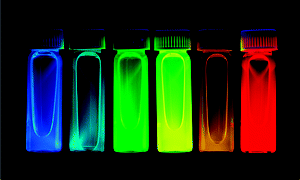
\includegraphics[width=0.35\linewidth]{quantum-dot} \\
	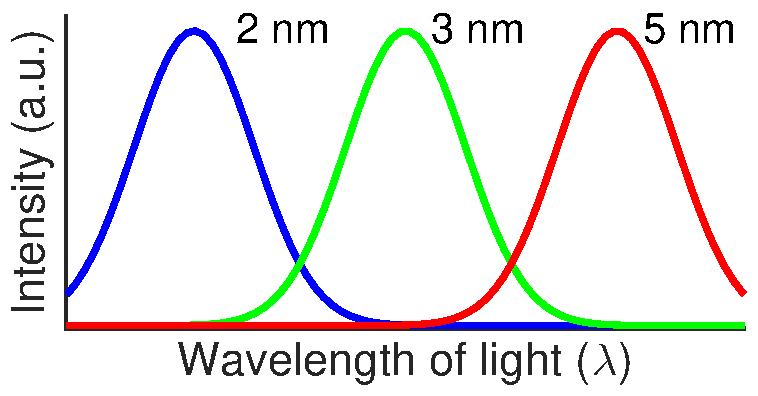
\includegraphics[width=0.42\linewidth]{quantum-dot-plot}
	\caption{The emission wavelength of cadmium selenide (CdSe) quantum dots can be tuned by changing the particle size. Smaller QDs, with radii from 2-\SI{3}{\nano\meter}, turn blue and green, while QDs with larger radii $\sim\SI{5}{\nano\meter}$ appear red. Top image reproduced from A. P. Alivisatos, \href{http://pubs.acs.org/doi/abs/10.1021/nn800485f1}{\emph{ACS Nano}}, \textbf{2008}, \emph{2}(8), 1514-1516.}
	\label{fig:qdot}
\end{figure}

Because of their tunable properties, QDs see many potential applications in transistors, solar cells, LEDs, diode lasers, and medical imaging.\footnote{There are many introductory articles out there on QDs, such as this editorial from \href{http://www.nature.com/nnano/journal/v5/n6/full/nnano.2010.127.html}{\emph{Nature Nanotechnology}} \textbf{5}, 381 (2010) and this article from J. Ouellette, \href{https://blogs.scientificamerican.com/cocktail-party-physics/quantum-dots-of-many-colors/}{\emph{Scientific American}}, 2012.} There's a lot of exciting research out there surrounding these nanoscale materials, whose functionality you should better understand having read this chapter!

%%%%%%%%%%%%%%%%%%%%%%%%%%%%%%%%%%%%%%%%%%%%%%%%%%%%%%%%%%%%%%%%%%%%%%%%%%%%%%%%

\section{Summary}
To recap, we dedicated this entire chapter to developing and analyzing the particle in a box quantum model. This simplistic, yet powerful assumption allowed us to solve the \Sch\ equation exactly, which revealed a set of stationary states and associated quantized energy levels. We demonstrated that the stationary state wave functions were orthogonal to each other, which allowed us to write the general solution to the \Sch\ equation as a superposition of stationary state solutions. We saw the complementarity of position and momentum manifest in the uncertainty principle, and we ended the chapter with a discussion of quantum dots, which are well-approximated by the particle in a box model. As we move on to more complex scenarios, we will be relaxing some of the strict assumptions we made in this chapter and exploring different potential functions. First, we will see what happens when we have a \emph{finite} potential barrier, which causes a peculiar phenomenon known as quantum tunneling.


%} % for doublespacing
%\end{document}